\section{Opis okruženja}

Simulacijsko okruženje će biti Carla zato što ima vrlo široko programsko sučelje za upravljanje aspektima simulacije te je besplatno za korištenje. Simulator se pokreće kao poslužitelj te se vozila dodaju pomoću skripte koja je napisana u programskom jeziku python.

\begin{figure}[ht!]
  \centering
  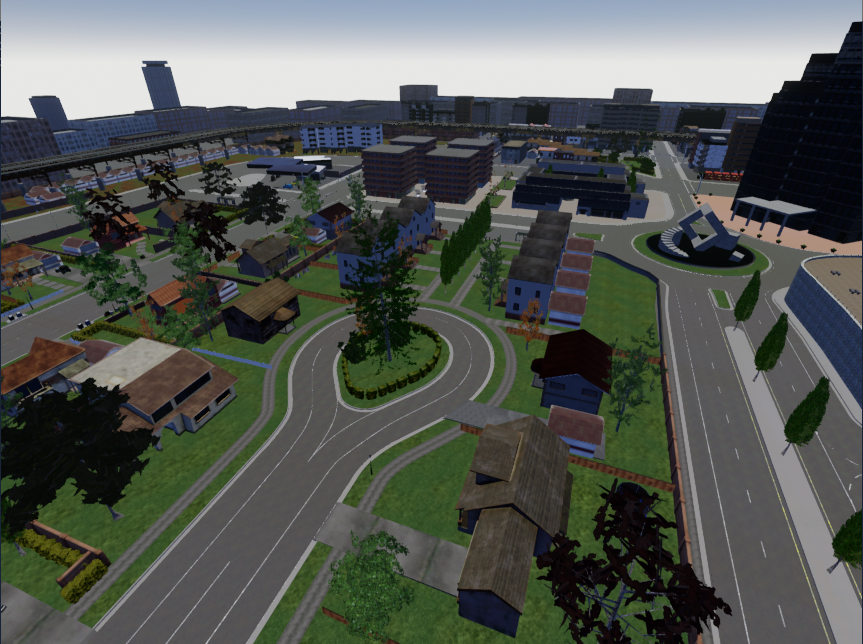
\includegraphics[scale=0.5]{images/carla_town03_example.png}
  \caption{Primjer karte pod nazivom Town03}
  \label{fig:town03_exmaple}
\end{figure}

Na slici \ref{fig:town03_exmaple} se vidi pogled na jedan od 7 mapa iz perspektive slobodne kamere. Korištene mape su definirane OpenDrive standardom. Simulator podržava raznolike senzore. Svi ti senzori se mogu postaviti samostalno na mapu, ali su najkorisniji kada se postave na drugo vozilo.

\newpage
\subsection{Senzori}
\subsubsection{RGB senzor}
\begin{figure}[ht!]
  \centering
  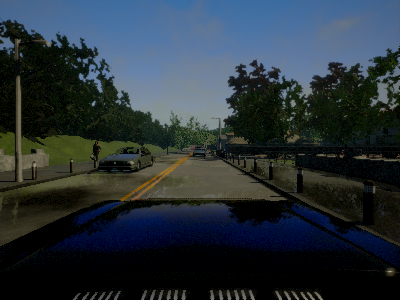
\includegraphics[scale=0.5]{images/rgb_example.png}
  \caption{Primjer regularne kamere\cite{carla:sensors}}
  \label{fig:rgb_exmaple}
\end{figure}

RGB senzor simulira kameru koja može snimati sliku koristeću crvenu, zelenu i plavu boju, tj. regularnu kameru. Ovaj senzor može prikupljati podatke iz simulatora u video obliku ili kao niz slika. Ovaj senzor se može koristiti u metodama lokalizacije koje kao temeljni algoritam koriste prepoznavanje ostalih sudionika u prometu prema obliku tj algoritmi prepoznavaju kontekst slike.

\subsubsection{Senzor dubine}
\begin{figure}[ht!]
  \centering
  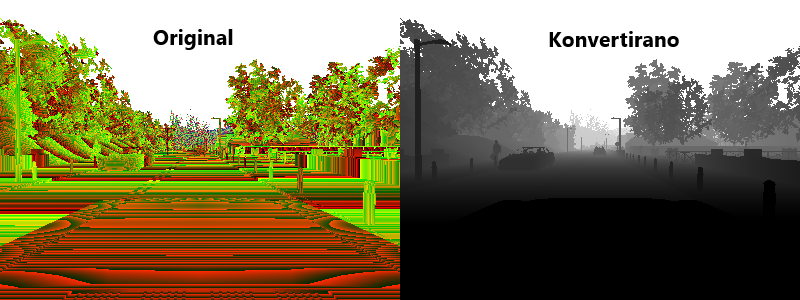
\includegraphics[scale=0.5]{images/depth_example.png}
  \caption{Primjer rezultata senzora dubine\cite{carla:sensors}}
  \label{fig:depth_exmaple}
\end{figure}

Ovaj senzor koristi nizove projicirajućih točaka da bi ilustrirao udaljenosti objekata, original na slici \ref{fig:depth_exmaple}. Tada se ti podaci pretvaraju u crno bijelu sliku gdje je svaki pixel u nijansama sive boje tj. ovisno koliko je objekt na određnome pixelu odaljen od kamere imati će svijetliju nijansu, konvertirano na slici \ref{fig:depth_exmaple}.

\newpage
\subsubsection{Semantičke segmentacije}
\begin{figure}[ht!]
  \centering
  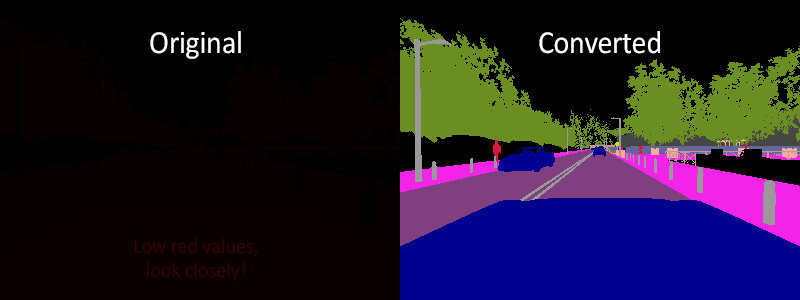
\includegraphics[scale=0.5]{images/sem_seg_exmaple.png}
  \caption{Primjer semantičke segmentacija\cite{carla:sensors}}
  \label{fig:sem_seg_exmaple}
\end{figure}

Ovaj senzor zapravo nije senzor ali je grupiran u klasu senzora zato što radi na vrlo sličan način kao i ostali senzori u simulatoru. Ovaj senzor dijeli sliku kamere na semantičke dijelove tj. objekte različitog tipa predstavlja drugim bojama. Na slici \ref{fig:sem_seg_exmaple} se vidi da je nebo crne boje, auti su plave boje, drveće je zeleno itd. OVaj način raspoznavanja objekata je moguć samo u simulator zato što nije potrebno razpoznavati objekte na slici već su oni definirani u simuliranoj okolini.

\subsubsection{LIDAR senzor}
\begin{figure}[ht!]
  \centering
  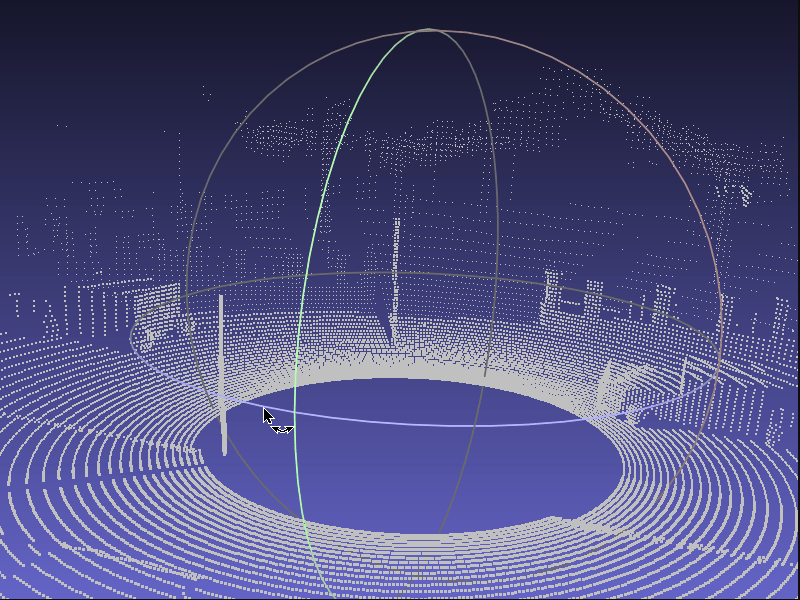
\includegraphics[scale=0.5]{images/LIDAR_examaple.png}
  \caption{LIDAR podaci\cite{carla:sensors}}
  \label{fig:lidar_exmaple}
\end{figure}
LIDAR (eng. light detecting and raging) senzor je zapravo vertikalan skup lasera koji simuliraju skeniranje od 360 stupnjeva tako da se rotiraju određeni broj puta u sekundi. Povratni podaci senzora su zapravo točke tj. koordinate relativne naspram samoga senzora do kojih su laseri uspjeli doći. Na slici \ref{fig:lidar_exmaple} se mogu vidjeti takvi podaci vizualizirani u programu MeshLab. Više o ulaznim parametrima senzora kasnije u radu.

\subsubsection{Senzor sudara}
Ovaj senzor dojavljuje klijentskome programu ako se vozila sudarilo s drugim objektom u simulaciji.

\subsubsection{Senzor prijelaza trake}
Ovaj senzor dojavljuje klijentskome programu ako je vozilo prošlo preko trake na cesti.

\subsubsection{GNSS senzor}
Senzor koji dojavljuje klijentskome programu trenutnu GNSS lokaciju vozila. Ta lokacija se interno računa tako da se lokacija vozila dodaje na geografsku referentnu lokaciju definiranu za cijelu mapu.

\subsubsection{Senzor prepreke}
Ovaj senzor javlja klijentskome programu ako se ispred vozila nalazi prepreka.

\subsection{Promet}
Postoji poveći broj već unaprijed definiranih vozila koja se mogu koristiti. Mogu se koristiti kao nositelji senzora ili kao ostali sudionici u prometu. Carla ima dobro definirana prometna pravila te semafore da bi simulacija izgledala što vjernije.
\newpage